The persistence API provides abstracted access to a persistence provider while
remaing decoupled from the underlying technology, including but not limited to
database, SQL version and transaction management, whilst employing a range of
software engineering tactics to concretely address required quality
requirements required for the peristence domain.

\subsection{Architecture Requirements}
The architectural requirements for the persistence API include the refined
quality requirements and architectural requirements listed below. The
architectural constraints for this lower level components are the same as for
the system as whole, as referred to in 
section \ref{sec:systemArchitecturalConstraints} with further extensions as
specified in section \ref{sec:persistenceAPIArchitecturalConstraints}.

\subsubsection{Access and Integration Requirements}
\subsubsection{Quality Requirements}
\paragraph{Flexibility}
The provided persistence API should be able to adapt to the rapidly evolving
persistence architecture domain, especially in terms of the different 
methodologies of storing data such as relational and NoSQL data stores. It is
further import that the persistence layer is not locked to any specific
persistence technology.

Further the chosen API should to force the use of any vender specific
transaction management, but should rather provide an abstraction layer allowing
the use of any transaction manager implementing the required interface.

\paragraph{Maintainability}
\label{sec:persistenceAPIMaintainability}
The used persistence API should be in a mature stage of the software development
lifecycle as to guard against a rapidly evolving changing API. The chosen
persitence API should be an open standard with multiple realization as to guard
against realization techologies be aboned. This will allow in future an easier 
switch to another persistence API implementaion if required for the long term
maintance and use of the project.

\paragraph{Scalability}
The chosen persistence API should be able to allow for future scaling of the
infrastrure either horizontally or vertically with a preference for 
horizontal scaling.

\paragraph{Performance}
The persitence API should allow for the use of certain architectural tactics
to increase performance. Specifically the following tactics should be supported
to some extent
\begin{itemize}
	\item Object Caching
	\item Connection Pooling
	\item Thread Provisioning
	\item Scheduling
\end{itemize}

\paragraph{Reliability}
The chosen API should allow security at least providing authorization on
entities managed by the underlying persistence technology architecture.

\subsubsection{Architectural Responsibilities}
The architectural responsibilities of the persistence API are shown in 
Figure \ref{fig:persistenceResponsibilities}
\begin{figure}[H]
	\begin{center}
	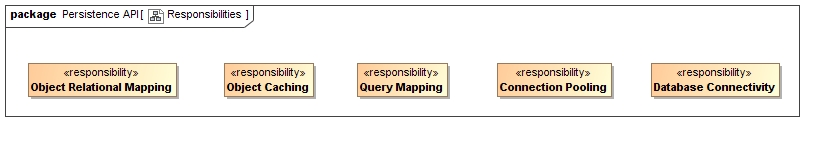
\includegraphics[scale=0.5]{../Diagrams and Charts/Persistence API/Responsibilities.jpg}
	\caption{The architectural responsibilities of the Persistence API}
	\label{fig:persistenceResponsibilities}
	\end{center}
\end{figure}

\subsubsection{Architecture Constraints}
\subsection{Architecture Design}
\subsubsection{Tactics}
\subsubsection{Architectural Components}
\subsubsection{Frameworks and Technologies}
\paragraph{Concrete Realization of Architectural Components}
\paragraph{Tactics}
\paragraph{Tools}
\paragraph{Concepts and Constraints for Application Components}